%----------------------------------------------------------------------------------------
%	PACKAGES AND OTHER DOCUMENT CONFIGURATIONS
%----------------------------------------------------------------------------------------

\documentclass{report}
\usepackage[english]{babel}
\usepackage[utf8]{inputenc}
\usepackage{fancyhdr} % Required for custom headers
\usepackage{lastpage} % Required to determine the last page for the footer
\usepackage{extramarks} % Required for headers and footers
\usepackage{graphicx} % Required to insert images
\usepackage{lipsum} % Used for inserting dummy 'Lorem ipsum' text into the template
\usepackage{subfigure} % Used for inserting figure side by side
\usepackage{amsfonts,amsmath,amssymb,amsthm}
\usepackage{array, hhline} % Table visual improvements
\usepackage{multirow}
%\usepackage{caption}
%\usepackage{subcaption}
\usepackage{hyperref} % Required to use hyperlinks

% block diagrams
\usepackage{tikz,textcomp}
\usetikzlibrary{shapes,arrows,matrix,fit}
\usetikzlibrary{circuits.ee.IEC}


% Margins
\topmargin=-0.45in
\evensidemargin=0in
\oddsidemargin=0in
\textwidth=6.5in
\textheight=9.0in
\headsep=0.25in 

\linespread{1.2} % Line spacing

\def\code#1{\texttt{#1}}

% Set up the header and footer
\pagestyle{fancy}
\lhead{\hmwkAuthorName} % Top left header
\rhead{\hmwkClass: \hmwkTitle} % Top center header
\chead{} % Top right header
\lfoot{} % Bottom left footer
\cfoot{} % Bottom center footer
\rfoot{Page\ \thepage\ of\ \pageref{LastPage}} % Bottom right footer
\renewcommand\headrulewidth{0.4pt} % Size of the header rule
\renewcommand\footrulewidth{0.4pt} % Size of the footer rule

\setlength\parindent{0pt} % Removes all indentation from paragraphs

%----------------------------------------------------------------------------------------
%	DOCUMENT STRUCTURE COMMANDS
%	Skip this unless you know what you're doing
%----------------------------------------------------------------------------------------

% Header and footer for when a page split occurs within a problem environment
\newcommand{\enterProblemHeader}[1]{
\nobreak\extramarks{#1}{#1 continued on next page\ldots}\nobreak
\nobreak\extramarks{#1 (continued)}{#1 continued on next page\ldots}\nobreak
}

% Header and footer for when a page split occurs between problem environments
\newcommand{\exitProblemHeader}[1]{
\nobreak\extramarks{#1 (continued)}{#1 continued on next page\ldots}\nobreak
\nobreak\extramarks{#1}{}\nobreak
}

\setcounter{secnumdepth}{0} % Removes default section numbers
\newcounter{homeworkProblemCounter} % Creates a counter to keep track of the number of problems

\newcommand{\homeworkProblemName}{}
\newenvironment{homeworkProblem}[1][Problem \arabic{homeworkProblemCounter}]{ % Makes a new environment called homeworkProblem which takes 1 argument (custom name) but the default is "Problem #"
\stepcounter{homeworkProblemCounter} % Increase counter for number of problems
\renewcommand{\homeworkProblemName}{#1} % Assign \homeworkProblemName the name of the problem
\section{\homeworkProblemName} % Make a section in the document with the custom problem count
\enterProblemHeader{\homeworkProblemName} % Header and footer within the environment
}{
\exitProblemHeader{\homeworkProblemName} % Header and footer after the environment
}

\newenvironment{homeworkSection}[1]{ % New environment for sections within homework problems, takes 1 argument - the name of the section
\renewcommand{\homeworkSectionName}{#1} % Assign \homeworkSectionName to the name of the section from the environment argument
\subsection{\homeworkSectionName} % Make a subsection with the custom name of the subsection
\enterProblemHeader{\homeworkProblemName\ [\homeworkSectionName]} % Header and footer within the environment
}{
\enterProblemHeader{\homeworkProblemName} % Header and footer after the environment
}
   
%----------------------------------------------------------------------------------------
%	NAME AND CLASS SECTION
%----------------------------------------------------------------------------------------

\newcommand{\hmwkTitle}{Final Course Project} % Assignment title
\newcommand{\hmwkClass}{Source Coding} % Course/class
\newcommand{\hmwkAuthorName}{Matteo Drago - 1151518} % Your name
\newcommand{\hmwkClassInstructor}{Giancarlo Calvagno} % Teacher/lecturer


%----------------------------------------------------------------------------------------
%	TITLE PAGE
%----------------------------------------------------------------------------------------
\begin{document}
\title{
\vspace{2in}
\textmd{\textbf{\hmwkClass \\ \hmwkTitle}}\\
\vspace{3in}
}
\author{\textbf{\hmwkAuthorName}}
\date{$21^{st}$ June 2018} % Insert date here if you want it to appear below your name

%----------------------------------------------------------------------------------------

\maketitle
\pagenumbering{gobble} % Used to delete the page number on the title page
\pagenumbering{arabic} % Used to reset the page number after the title page
\setcounter{page}{1}

\clearpage 

\section{Abstract}
In this project I built \textbf{coding} and \textbf{decoding} procedures for static color images by means of vector quantization. In order to do this I implemented the quantizer using the \textit{Linde Buzo Gray} algorithm, in the \textit{split} version; the rate \textit{R} will be of 8 bit/pixel for vectors of size \textit{L} = 3, where the three components are the (R,G,B) or the (Y,U,V) representation of the color image at 8x3 bit/pixel.

In the following, after a brief theory overview and the description of few choices in the procedure to build the algorithm, I will compare the performance in terms of distortion and PSNR with respect to the results obtained with the JPG standard.

\section{Data Compression}
The two main components that defines a compression system are:
\begin{itemize}
	\item the \textbf{encoder} which takes as input the message $\mathcal{A}$ (it could be text, image or audio) and produces its coded version, $\mathcal{A}'$;
	\item the \textbf{decoder} which, upon receiving $\mathcal{A}'$, tries to reconstruct the original message $\mathcal{A}$.
\end{itemize}   
The \textit{type} of quantization depends on the technique implemented by our encoder/decoder pair; we speak of \textbf{lossless} compression when the decoder is able to perfectly reconstruct the message $\mathcal{A}$ from $\mathcal{A}'$. However, if we want to achieve an higher level of compression we have to pay in terms of reconstruction quality at the receiver side and in this case we speak of \textbf{lossy} compression: the receiver is not able to recreate the original message $\mathcal{A}$, but it provides a lower quality version.

While for the lossless compression we evaluate the performances just in terms of \textbf{rate} (i.e. the average number of bits used to represent each sample value), in the lossy scenario we need also to evaluate how much the received message differs from the original one: this metric is called \textbf{distortion}. The relation between these two metrics is described with the \textit{rate-distortion} \cite{rate_dist} theory, a set of rules and guidelines that let us determine, for example, the minimum rate that we can guarantee to the system without exceeding a certain amount of distortion.

Given the two different versions of the same message, how can we actually measure the distortion between them? We can use the \textit{squared error} between the input sequence \textbf{\textit{x}} and the reconstructed one \textbf{\textit{y}}, defined as $(x-y)^2$; in alternative we can use the \textit{absolute difference} defined as $|x-y|$. In general, however, average measures are more informative, and in fact we use the \textit{mean squared error}:
\begin{equation}
\sigma^2_d = \frac{1}{N} \sum_{n = 1}^{N} (x_n - y_n)^2
\end{equation}
which appears also in another useful metric, the \textit{signal-to-noise ratio}:
\begin{equation}
SNR(dB) = 10log_{10}\frac{\sigma^2_x}{\sigma^2_d}
\end{equation}
where $\sigma^2_x$ is the average squared value of the original message. In the image processing domain there's another important quantity related to the \textit{MSE}, which is the \textit{peak-signal-to-noise ratio} defined as: 
\begin{equation}
PSNR(dB) = 10log_{10}\frac{x^2_{peak}}{\sigma^2_d} 
\end{equation}
where $x_{peak}$ is the peak value assumed by the original signal. I'm going to use these measures to quantify the quality of the reconstructed image and to discuss the results, in the dedicated section.

Another way for categorizing our compression system is to consider the type of quantization implemented; if it applies \textbf{scalar} quantization, we have to code one source symbol at a time; using \textbf{vector} quantization instead, it codes groups of symbols altogether, with the advantage of obtaining lower distortion for a given rate (or vice versa, a lower rate for a given limited distortion). % As I outlined in the introduction, the aim of this project is the design of a version of the \textbf{LBG} algorithm, which finds a set of representative L-dimensional vectors, that constitute the \textit{codebook} for our vector quantizer. Once the codebook is complete, it is stored both at the encoder and at the decoder side. % in this way, the encoder has just to find the closest code-vector to the pixels and to assign to each pixel the corresponding index of word in the codebook; then, we send through the channel the list of indexes and, once received, the decoder has to do just a table look-up in order to convert the indexes again in the corresponding pixel values.

\section{The Linde-Buzo-Gray algorithm}

Before delving into details, I would like to highlight that the main task of the project is \textbf{codebook} evaluation: all the computational efforts are focused in finding the optimal set of \textbf{L-dimensional} vectors that minimizes the distortion at the receiver, for a given rate \textbf{R}. Once the codebook is complete, we assume that it is stored both at the encoder and at the decoder side.

One way of implementing the procedure is firstly to assume the distribution function of the input data $f_X(x)$ as known:  the first step is a suitable initialization of the codebook, and the optimal repartition of input samples $ x \in \mathbb{R}^L$. Using our knowledge of $f_X(x)$ we recompute the codebook, then we assign to each sample the best codeword and we evaluate the distortion $D^{(n)}$ (where \textit{n} indicates the number of iteration in sequential order). This procedure iterates until the following stopping condition is verified: 
\begin{equation}
\frac{D^{(n-1)} - D^{(n)}}{D^{(n)}} < \epsilon
\end{equation}
where $\epsilon$ is an arbitrary small design parameter. Note that this algorithm guarantees that the distortion \textbf{never increases}, even if it may not be globally minimized.

In our case, however, the probability distribution function is not known a-priori, and so the initial algorithm needs the following slight change: 

\begin{enumerate}
	\item Start from a codebook of size K. Set $n = 1$ and $ D^{(0)} = \infty $. Assign a suitable value to $\epsilon$; %\textbf{In this case all pixels are represented by this codeword}; 
	\item Partition the dataset with respect to the codebook: to each pixel is assigned the nearest codeword;
	\item Compute the new codewords as centroids of the clusters:
	\begin{equation}
	c_i^{(n)} = \frac{1}{|C_i^{(n)}|} \sum_{x \in C_i^{(n)}} x \quad i = 1,...,K
	\end{equation}
	\item Evaluate the new distortion value:
	\begin{equation}
	D^{(n)} = \frac{1}{|\mathcal{P}|} \sum_{x \in \mathcal{P}} ||x - c_x^{(n)}||_2^2
	\end{equation}
	where $c_x^{(n)}$ is the codeword assigned to the pixel \textbf{\textit{x}} a the n-th iteration.
	\item If the termination condition described in (4) is met, the computation stops, otherwise increase \textit{n} by one and return to step 2.
\end{enumerate}

We can notice that there are several similarities with the Lloyd's algorithm \cite{Lloyd}, which is also used in pattern recognition when we want to subdivide a dataset of points into \textit{k} representative clusters (in our case we can think of the codebook as a set of centres for the different clusters). As for the Lloyd's algorithm, also in our case the codebook initialization is fundamental to guarantee that the algorithm converges to an optimum in considerably less iterations and computational efforts (for a good Lloyd's initialization technique, see \textit{kmeans++} \cite{kmeans++}). In past years several techniques were implemented with the aim of optimizing this step and in this project I will focus on the \textbf{splitting technique}, where initially we start with a codebook of size 1 (same codeword assigned to each pixel). Then, the second codeword is obtained as $ c_2 = c_1 + \delta$ and LBG is performed on the new codebook; when LBG finishes, we can double the size of the codebook simply using $c_{2i} = c_i + \delta$. We can iterate this procedure until we reach the desired codebook size (and of course we can also obtain sets of odd dimensions, by simply deciding how many additional codewords to create). The reason behind this "iterative doubling" lies on the fact that at each iteration we are sure to start from the optimal version of the codebook, thank to the optimality property of LBG.

\section{MATLAB implementation}

%The \textit{end-to-end} environment that I wrote consists of one main script \code{main.m} and three distinct auxiliary functions. 
In this case, the decision of how to pre-process data is fundamental: I decided to import raw image and work with their RGB representation; in particular I haven't used the \code{uint8} format for the pixels, but I used the \code{im2double} routine instead, in order to avoid mathematical problems (it normalizes the interval from [0 255] to [0 1], original values are reconverted in the end).

Coding the procedure described in the previous section required to address with different issues; first of all, the well-known \textbf{empty cell} problem. It may happen that, at some point of LBG, one codeword has no pixels assigned (its cluster is empty) and it can be seen as an \textit{outlier} of the pixel distribution. In MATLAB I had to avoid this condition because when trying to compute the centroid of each cluster it results in triplets of \code{NaN}.

The routine \code{checkAnyEmptyClt.m} tries to avoid this problem: it checks if there are any empty sets during a particular iteration. This checking operation, however, takes time if not properly optimized and, after testing different solutions, I decided to use the MATLAB function \code{tabulate}, which takes as input a column array of size \textit{widthX height} (parameters of the input image). Each position of the array represents one pixel and it assumes the index of the respective codeword in the codebook; the output of the function gives complete information on how the array is populated so, after few adjustments, in the end the routine returns the index of the \textbf{first} empty cluster on the list. 

Of the course the correspondent codeword must be substituted and, in order to do so, I decided to use as candidates the pixels of the \textit{most populated} cluster; a new codeword is picked randomly from this set and after that all clusters are updated consequently. This step is crucial to understand my implementation of LBG, which can be found in the function \code{LBG.m}: in fact, the algorithm persists on point \textbf{2} described above until all clusters are populated; once all codewords have \textit{at least one} assigned pixel, the procedure can continue from point \textbf{3}.

In general, LBG assigns to a pixel the \textbf{nearest} codeword, which is the one that provides the smaller distortion. Here instead, I decided to write \code{LBG.m} such that a codeword is assigned to a pixel only if: 
\begin{equation}
D_{new} < GD_{old}
\end{equation}
where $D_{new}$ is the distortion between the pixel and the new candidate codeword, $D_{old}$ considers the current assigned codeword and $\mathbf{G}$ is a design parameter to set at the beginning of the simulation. After different tests, I confirmed that this design choice guarantees that the algorithm doesn't get stuck on situations where one pixel keeps on switching from one cluster to another increasing the number of iterations (and so the execution time) without providing any valuable improvement; in fact with this small modification one pixel changes cluster only if using a different codeword introduces a \textbf{\textit{considerable}} gain. The final choice of \textbf{G} is done considering that also a value too small leads to the problem of coarse approximation (few updates, higher distortion), and so we need to find a good trade-off between the number of iterations and the quality of results (the standard LBG comes with $G = 1$).
Another possibility, if one wants to avoid the code to be stuck in a loop, is to set a maximum number of iterations after which the algorithm exits the cycle.
I've written also the function \code{distortion.m}, in order to speed up time performances in evaluating the euclidean distance between triplets of pixels.

Once finished with the codebook evaluation we can code the image appropriately: considering the described design, we just need to rearrange the column array representing codebook indexes, in order to build the output image. These indexes are then translated in real pixels at the decoder side, and so we can compare the quality between input and output version of the image.

Just to sum up, the steps are the following:
\begin{itemize}
	\item Image preprocessing and parameters initialization
	\item Codebook evaluation via LBG split
	\item Coding of the image into its quantized version
	\item Study of the differences with the original image
\end{itemize}

\begin{figure}
	\subfigure[Codebook size = 2]
	{
		\includegraphics[scale=.4]{img/1/img_png_1}
	}
	\hfill
	\subfigure[Codebook size = 4]
	{
		\includegraphics[scale=.4]{img/1/img_png_2}
	}
	\hfill
	\subfigure[Codebook size = 8]
	{
		\includegraphics[scale=.4]{img/1/img_png_3}
	}
	\hfill
	\subfigure[Codebook size = 16]
	{
		\includegraphics[scale=.4]{img/1/img_png_4}
	}
	\vfill
	\subfigure[Codebook size = 32]
	{
		\includegraphics[scale=.4]{img/1/img_png_5}
	}
	\hfill
	\subfigure[Codebook size = 64]
	{
		\includegraphics[scale=.4]{img/1/img_png_6}
		\label{fig:complete_1e}
	}
	\hfill
	\subfigure[Codebook size = 128]
	{
		\includegraphics[scale=.4]{img/1/img_png_7}
	}
	\hfill
	\subfigure[Codebook size = 256]
	{
		\includegraphics[scale=.4]{img/1/img_png_8}
		\label{fig:complete_full}
	}
	\caption{256x256 quantized image - $\epsilon = 0.001$, $G = 1$ and $\delta = 0.2$}
	\label{fig:complete_1}
\end{figure}

\clearpage

\section{Performance Evaluation}
In order to test the algorithm and to evaluate performances, I used colour images from the dataset in \cite{SIPI}; all pictures are of size 256x256 or 512x512, I didn't test images of higher dimension because the only difference is on the execution time and not on real coding performances. All the dataset images are of type TIFF, suitable for our purposes; finally, after few tests I decided to set $\delta = 0.2$.

Just to give an insight on all intermediate iterations, Figure \ref{fig:complete_1} shows what the quantized image looks like using different codebook sizes, from 2 up to 256. It's clear how the quantization gains in precision as we increase the number of clusters: even if the face and different edges are clearly distinguishable using just 6 bit/pixel (Figure \ref{fig:complete_1e}), the shadows and colour shades of scarf and flowers are appreciable just with higher rates.

Before further discussions, it could be useful to spend few additional words on the meaning of \textit{rate} in this contest, with the intention of keeping my considerations consistent. First of all, we should remember that at the beginning our image is a matrix of (R,G,B) triplets representing pixels; each channel can assume values from 0 to 255, and so each pixels correspond to 24 bits of information (8 bit per channel). Thus, in our scenario the \textit{rate} is the number of bits that we have to use in order to represent one single pixel (in fact we use \textbf{compression} exactly to reduce this quantity). The main point of the LBG procedure is that, if we assume the codebook as stored both at the encoder and decoder sides, we just need to send the corresponding index of the codeword for each single pixel: in our case, given that the maximum codebook size is 256, we need at most 8 bits to represent each index. 

\begin{figure}
	\begin{minipage}[b]{0.55\textwidth}
		\centering
		\subfigure[]
		{
			\includegraphics[width=\linewidth]{img/1/distortion}
			\label{fig:comparison_dist}
		}
		
		\vspace*{3mm} % vertical whitespace
		\subfigure[]
		{
			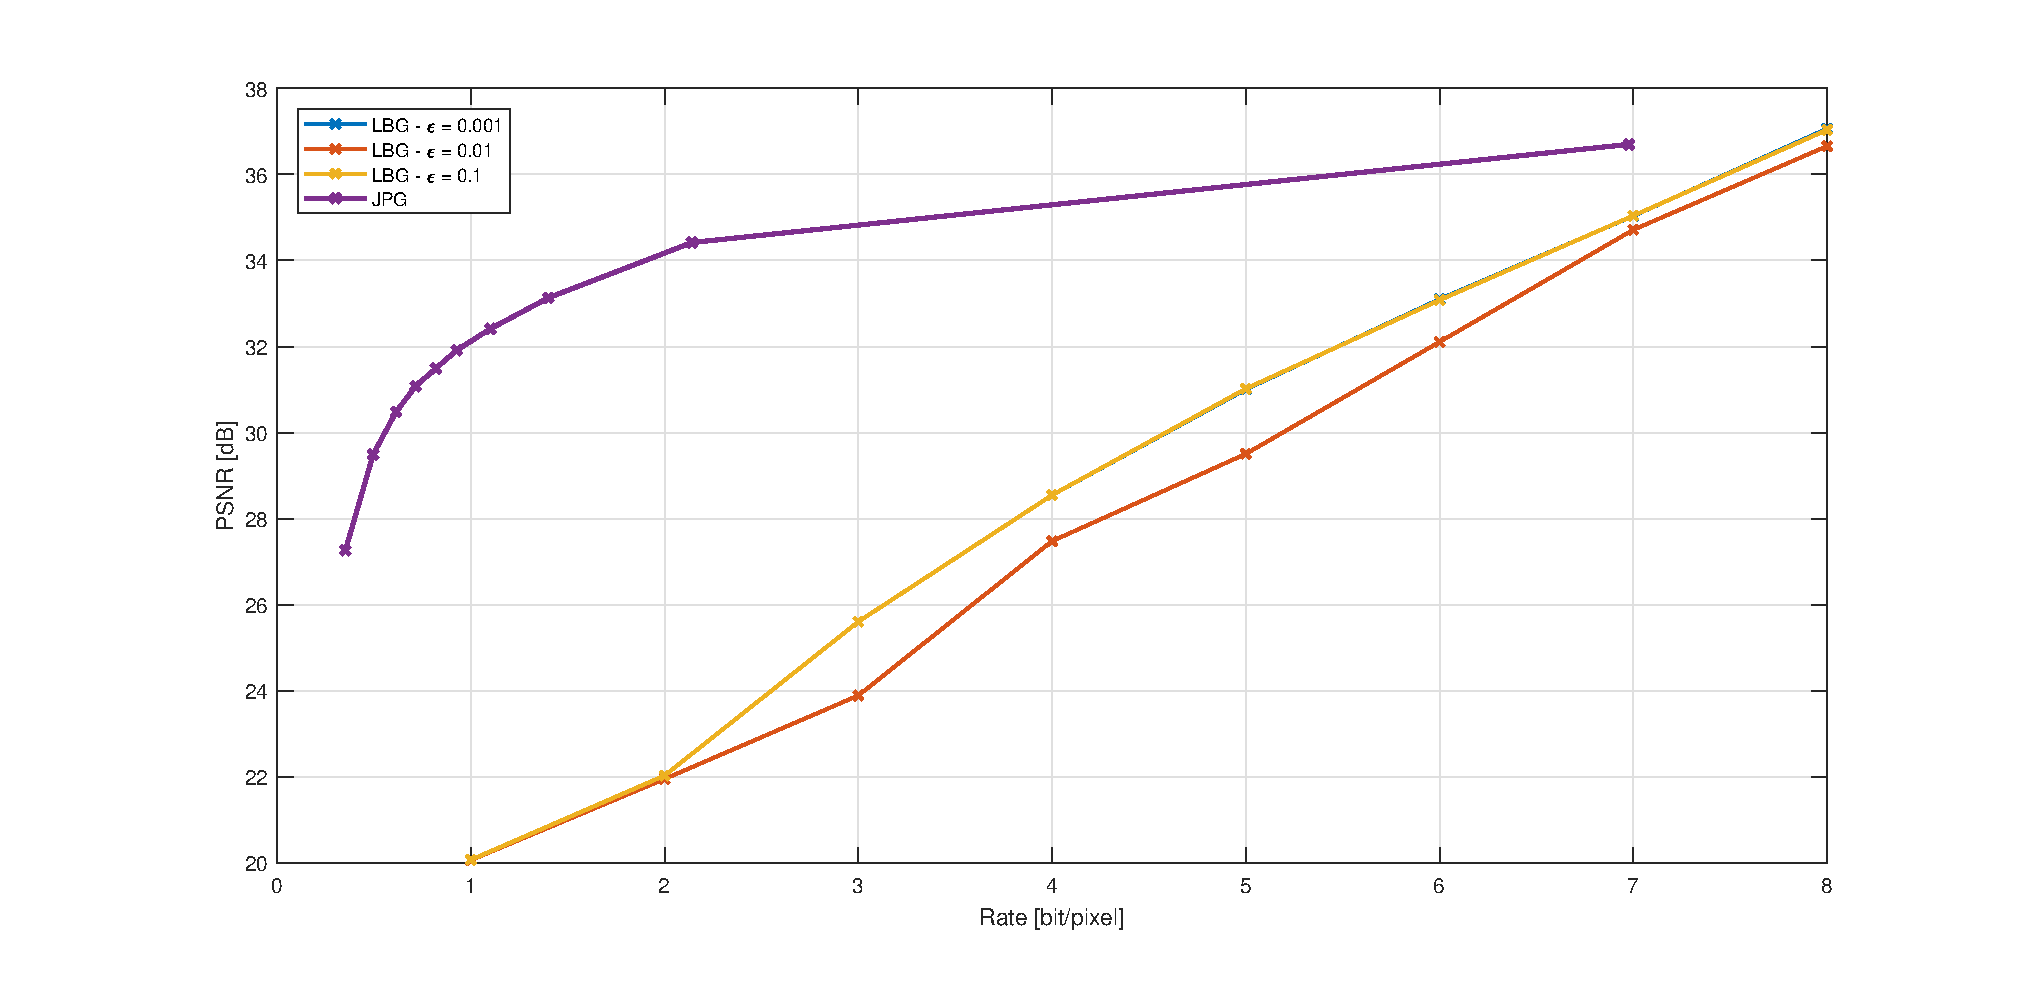
\includegraphics[width=\linewidth]{img/1/psnr}
			\label{fig:comparison_psnr}
		}
	\end{minipage}
	\hfill        % horizontal whitespace
	\subfigure[]
	{
		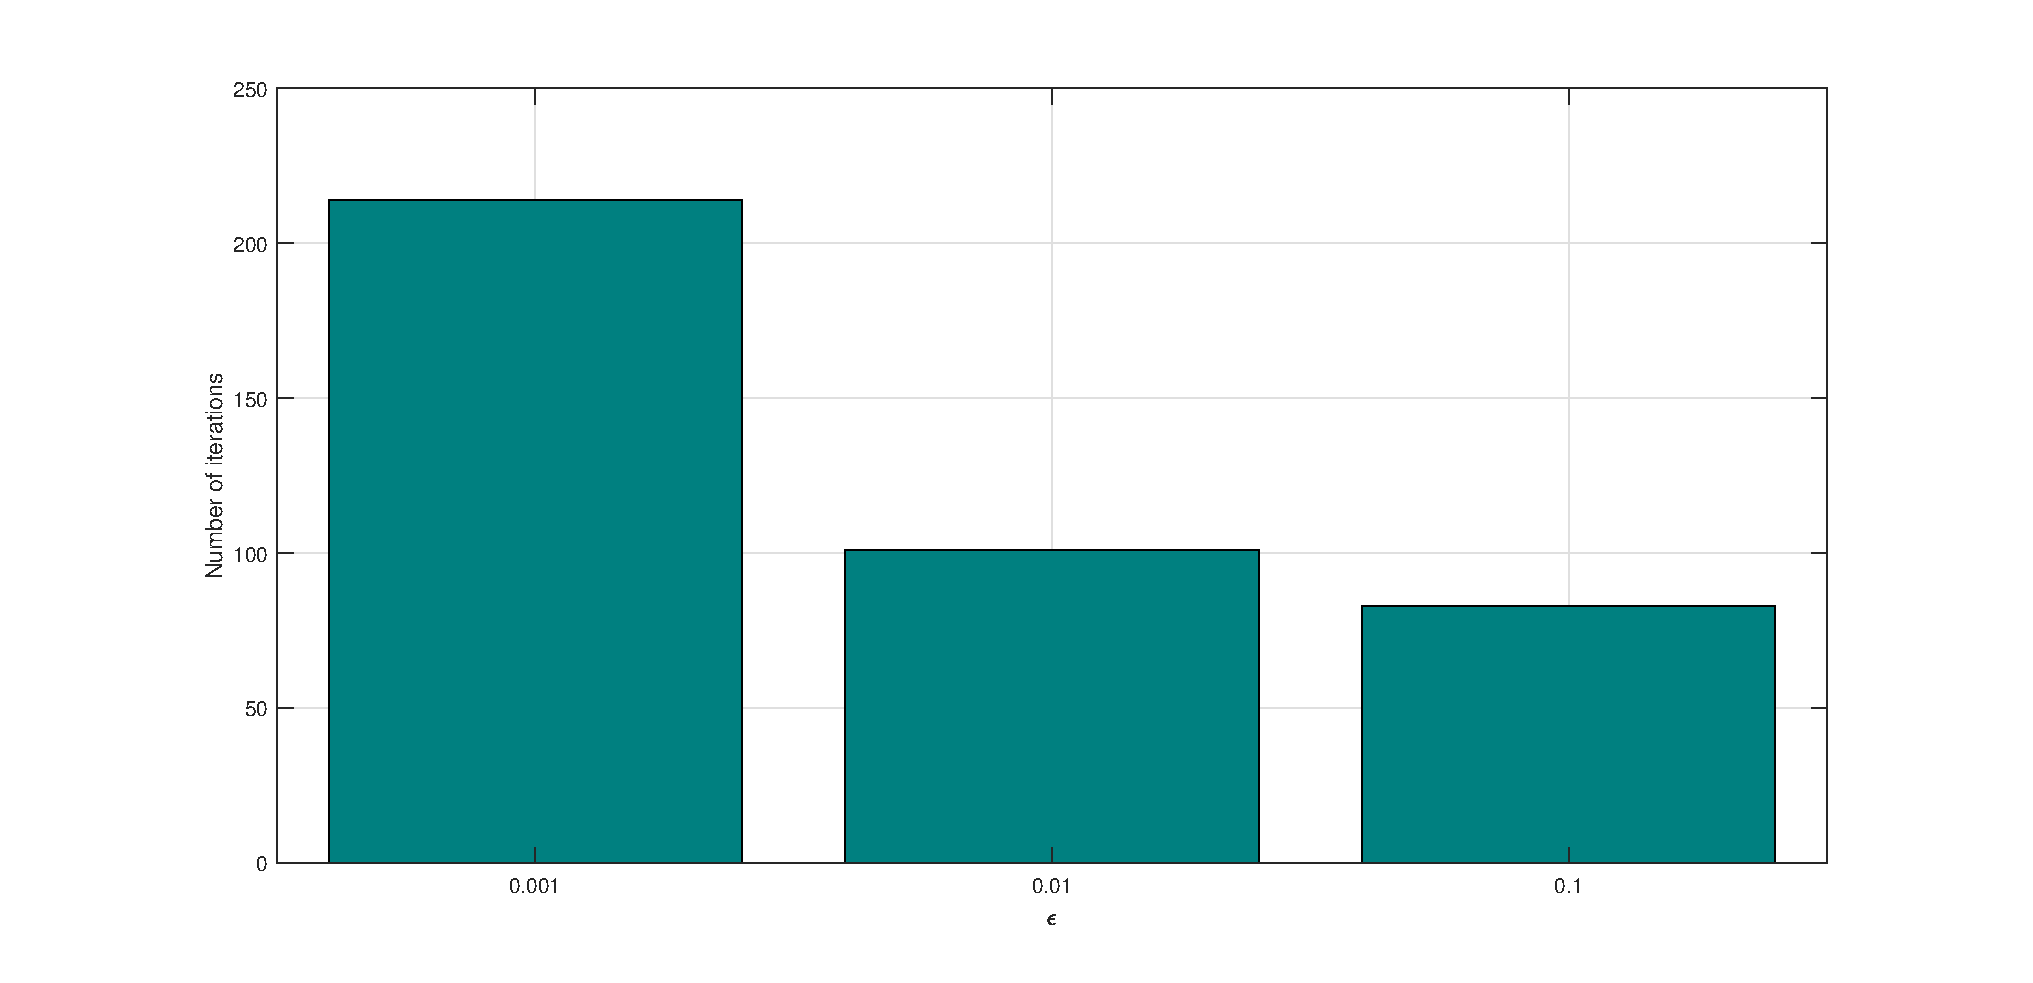
\includegraphics[width=0.45\linewidth, height=0.6\linewidth]{img/1/iterations}
		\label{fig:iterations_1}
	}
	\caption{Comparison of distortion and PSNR for the image at \ref{fig:complete_full}}
	\label{fig:comparison_1}
\end{figure}
 
Considering that, in Figure \ref{fig:comparison_1} I compared PSNR and distortion (as defined is the second section) in function of the rate and for different values of $\epsilon$. We can see how, with this particular picture, using a lower $\epsilon$ increases performances, especially at lower rates; changing from $\epsilon = 0.01$ to $0.001$ however doesn't seem to provide any advantage, but instead it just increases the price that we have to pay in terms of number of \textit{overall iterations} of the procedure, as shown in Figure \ref{fig:iterations_1}. 

In Figures \ref{fig:comparison_dist} and \ref{fig:comparison_psnr} it is shown also what changes if we use JPG compression \cite{jpeg} (the parameter \code{Quality} of the MATLAB tool has been used with value from 1 to 100): it's clear that in any case JPG provides higher quality with the same rate (and in the JPG scenario we send the compressed image all at once). The price that we have to pay, not only in terms of bit/pixel but also in terms of computational time, in order to have few dB of gain in PSNR (or lower MSE in terms of distortion) using LBG with respect to JPG doesn't motivate the choice of first method with respect to the latter.

\begin{figure}[ht]
	\centering
	\subfigure[]
	{
		\includegraphics[scale=.4]{img/1/cloud}
		\label{fig:cloud_1}
	}
	\hfill
	\subfigure[Image Palette]
	{
		\includegraphics[scale=.5]{img/1/palette}
		\label{fig:palette_1}
	}
	\caption{}
\end{figure}

In Figure \ref{fig:cloud_1} I provided a 3D visualization of the image where each axis represents one of the (R,B,G) channels. I found really interesting to see how different codewords are distributed among the cloud of points: as a confirmation of all previous considerations we can notice how where the cloud is more dense of pixel we need more codewords to represent this high variability while, where the cloud is sparse, few codewords are needed. 

It's been curious also to find a way to visualize the image palette obtained from the codebook with the aim of making it look \textit{as continuous as possible}. In the end I decided to start from the codeword with the minimum value in one of the selected channels and to stack consecutively codewords that minimize the Euclidean distance from the last inserted point; \cite{sort_color} and \cite{disney_color_kingdom} make a really interesting in-depth analysis of the problem. 

I decided to put in this report also some other tests using different representative images and lower values of \textbf{G}. It was interesting to see that in Figure \ref{fig:analysis_8} for example the JPG compression needs even less bits to represent one pixel than in the previous case, and this is probably due to the fact that the image presents a plain background; this is confirmed also by the palette of Figure \ref{fig:palette_8} that shows lot of codewords (and so, colours) similar to each other.

The surprise came with the results of Figure \ref{fig:analysis_8}: in this case the LBG algorithm seems to perform better than the JPG! In fact after a certain point JPG needs an higher rate in order to guarantee a given required quality, while LBG manage to provide higher quality at a lower rate. The reason behind this behaviour could be the high level of details of Figure \ref{fig:quant_10}: we can see in fact that there are many variations on colour shades, also due to the many edges that characterize the baboon face. Moreover, in Figure \ref{fig:cloud_10} we can appreciate how well the codebook approximates the cloud of points: also this could be a qualitative measure of the quality of the designed algorithm. Despite this isolated case, I'm confident to say that LBG is not to be preferred to JPG (considering execution time). 

We need also to highlight that in all tests (also in Figure \ref{fig:analysis_4}) there aren't considerable changes or improvements in using lower values of $\epsilon$: thus, as highlighted before, when possible we should choose for the path that leads to the lower computational complexity.

\section{Conclusions}
I found this project really interesting and stimulating. Deciding different trade-off between computational time, quality of quantization and complexity of the algorithm has been very challenging and helped me understand pros and cons of the different techniques. In the end, it seems to me pretty clear that the choice should fall on JPG, for the reasons that I described in detail previously. However, LBG could be a good comparison metric, given the assumption of optimality of the procedure.

\begin{figure} 
	\centering
	\subfigure[256x256 quantized image - $\epsilon = 0.1$, $G = 0.8$ and $\delta = 0.2$]
	{
		\includegraphics[width=.2\linewidth]{img/4/img_png_8}
	}
	\hfill
	\subfigure[Image Palette]
	{
		\includegraphics[width=.2\linewidth]{img/4/palette}
	}
	\hfill
	\subfigure[Cloud of pixels]
	{
		\includegraphics[width=.75\linewidth]{img/4/cloud}
	}
	\vfill
	\subfigure[Distortion vs Rate]
	{
		\includegraphics[width=.6\linewidth]{img/4/distortion}
	}
	\hfill
	\subfigure[PSNR vs Rate]
	{
		\includegraphics[width=.6\linewidth]{img/4/psnr}
	}
	\caption{Complete analysis of "Woman on Grey Background"}
	\label{fig:analysis_4}
\end{figure}

\begin{figure} 
	\centering
	\subfigure[256x256 quantized image - $\epsilon = 0.1$, $G = 0.9$ and $\delta = 0.2$]
	{
		\includegraphics[width=.2\linewidth]{img/8/img_png_8}
	}
	\hfill
	\subfigure[Image Palette]
	{
		\includegraphics[width=.2\linewidth]{img/8/palette}
		\label{fig:palette_8}
	}
	\hfill
	\subfigure[Cloud of pixels]
	{
		\includegraphics[width=.75\linewidth]{img/8/cloud}
	}
	\vfill
	\subfigure[Distortion vs Rate]
	{
		\includegraphics[width=.6\linewidth]{img/8/distortion}
	}
	\hfill
	\subfigure[PSNR vs Rate]
	{
		\includegraphics[width=.6\linewidth]{img/8/psnr}
	}
	\caption{Complete analysis of "Sparse Smarties"}
	\label{fig:analysis_8}
\end{figure}

\begin{figure} 
	\centering
	\subfigure[256x256 quantized image - $\epsilon = 0.01$, $G = 1$ and $\delta = 0.2$]
	{
		\includegraphics[width=.2\linewidth]{img/10/img_png_8}
		\label{fig:quant_10}
	}
	\hfill
	\subfigure[Image Palette]
	{
		\includegraphics[width=.2\linewidth]{img/10/palette}
	}
	\hfill
	\subfigure[Cloud of pixels]
	{
		\includegraphics[width=.75\linewidth]{img/10/cloud}
		\label{fig:cloud_10}
	}
	\vfill
	\subfigure[Distortion vs Rate]
	{
		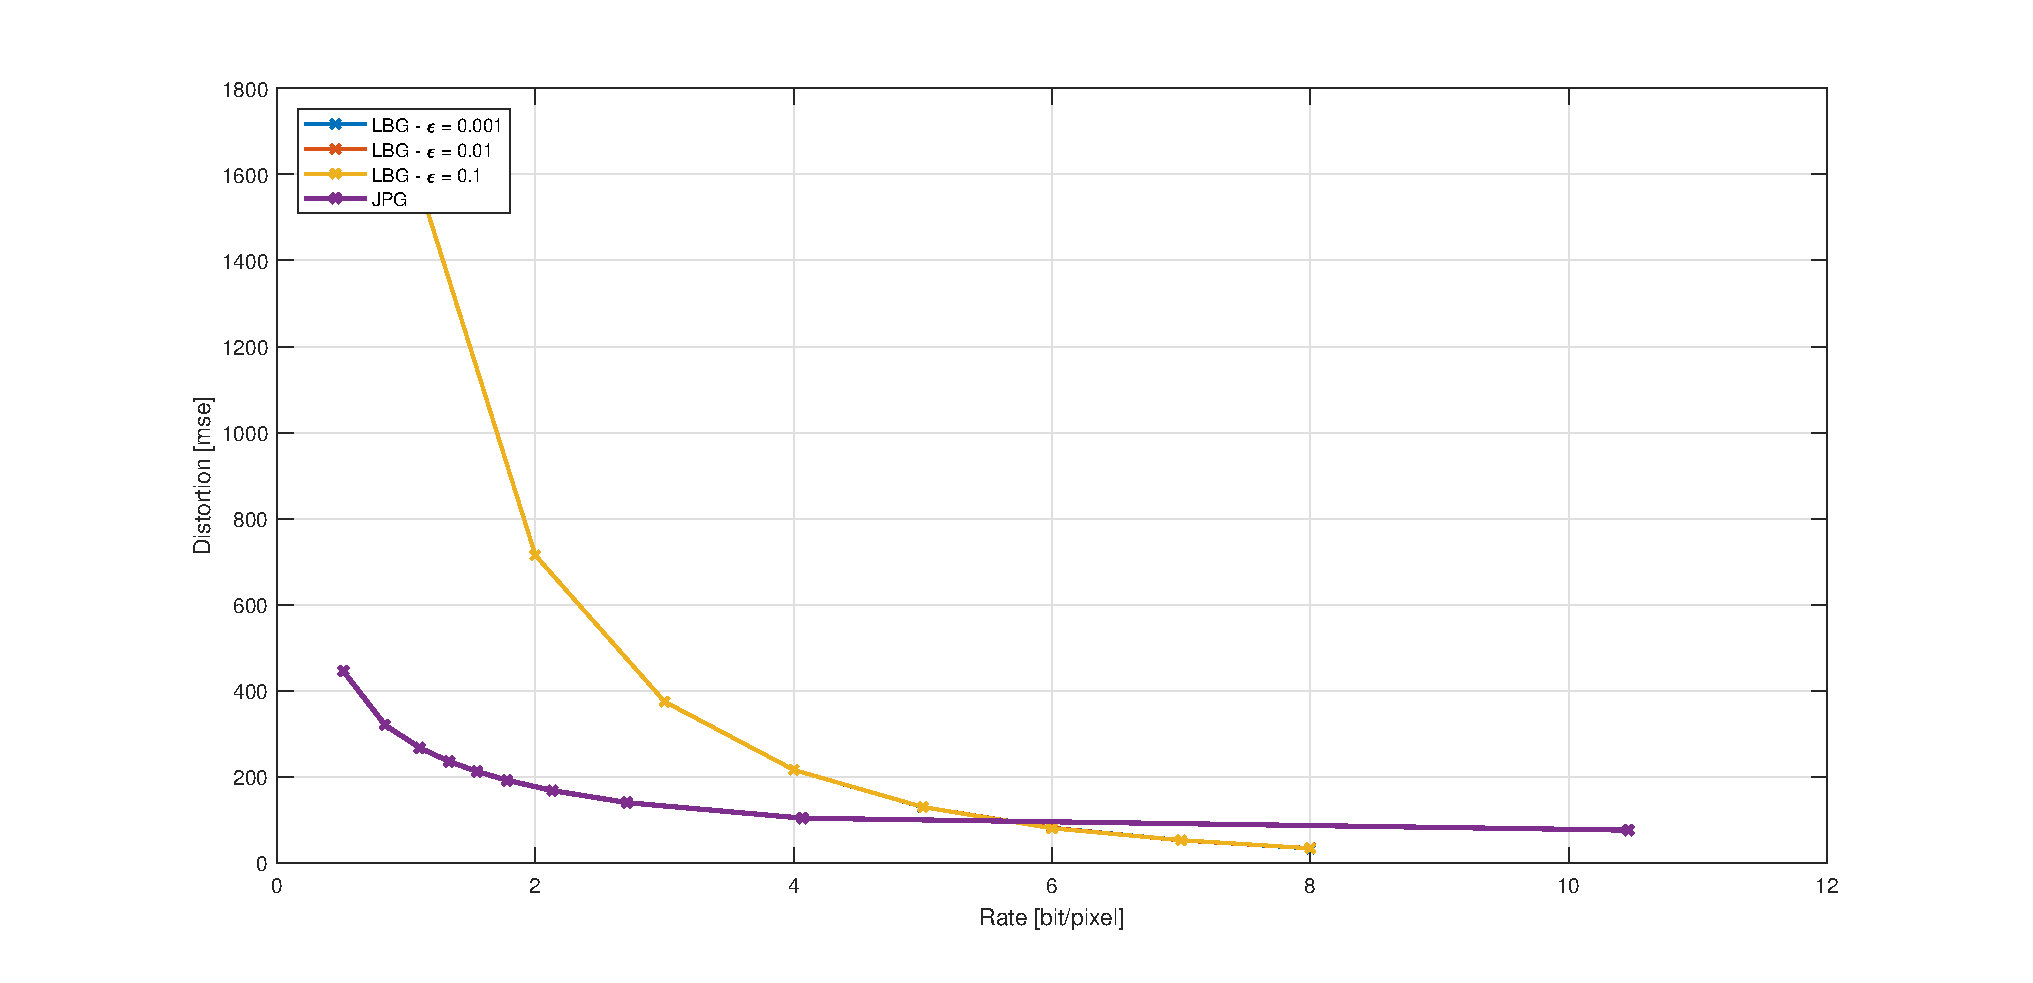
\includegraphics[width=.6\linewidth]{img/10/distortion}
	}
	\hfill
	\subfigure[PSNR vs Rate]
	{
		\includegraphics[width=.6\linewidth]{img/10/psnr}
	}
	\caption{Complete analysis of "Baboon"}
	\label{fig:analysis_10}
\end{figure}

\clearpage

\begin{thebibliography}{9}
		
	\bibitem{rate_dist}
		\textit{Rate Distortion Theory: A Mathematical Basis for Data Compression}
		Tony Berger (1971), Prentice Hall
		
	\bibitem{Lloyd}
		\textit{Least squares quantization in PCM}
		Lloyd, Stuart P. (1982), IEEE Transactions on Information Theory
		
	\bibitem{kmeans++}
		\textit{k-means++: The Advantages of Careful Seeding}
		David Arthur and Sergei Vassilvitskii (2007)
		
	\bibitem{SIPI}
		\textit{SIPI Image Database},
		USC, University of Southern California
	
	\bibitem{TIFF}
		\textit{Tagged Image File Format},
		\href{https://it.wikipedia.org/wiki/Tagged_Image_File_Format}{Wikipedia webpage}
	
	\bibitem{jpeg}
		\textit{The JPG still picture compression standard}
		G.K. Wallace, Digital Equipment Corp., Maynard, MA, USA
		
	\bibitem{sort_color}
		\textit{The incredibly challenging task of sorting colours},
		\href{https://www.alanzucconi.com/2015/09/30/colour-sorting/}{https://www.alanzucconi.com/2015/09/30/colour-sorting/}
	
	\bibitem{disney_color_kingdom}
		\textit{A Visit to Disney’s Magic Kingdom},
		\href{	http://blog.wolfram.com/2013/08/13/a-visit-to-disneys-magic-kingdom/}{	http://blog.wolfram.com/2013/08/13/a-visit-to-disneys-magic-kingdom/}
		Theodore Gray, Co-founder, Wolfram Research, Inc; Founder, Touch Press; Proprietor, periodictable.com 
	
	
\end{thebibliography}

\end{document}